% \documentclass{article}
% \usepackage[utf8]{inputenc}
% \usepackage{graphicx}
% \usepackage{amsmath}
% \usepackage{url}
\graphicspath{{./images/}}

\title{CS 6000 Git Assignment}

\author{Katrina J. Rosemond}
\date{September 21, 2022}

%\begin{document}


\section{Introduction - Katrina Rosemond}

Hello, my name is Katrina Rosemond. I am a 3rd year Ph.D. computer science 
student at the University of Colorado Colorado Springs (UCCS). As a 
research assistant in the Embedded Systems Security Lab (ESSL), my 
research focuses on cyber-physical system (CPS) security, particularly 
automotive security. I earned my bachelor's degree in electrical 
engineering from NC A\&T State University. However, I found a passion for 
hardware and software, leading me to pursue a computer science graduate 
degree. 

\begin{figure}[ht]
    \centering
    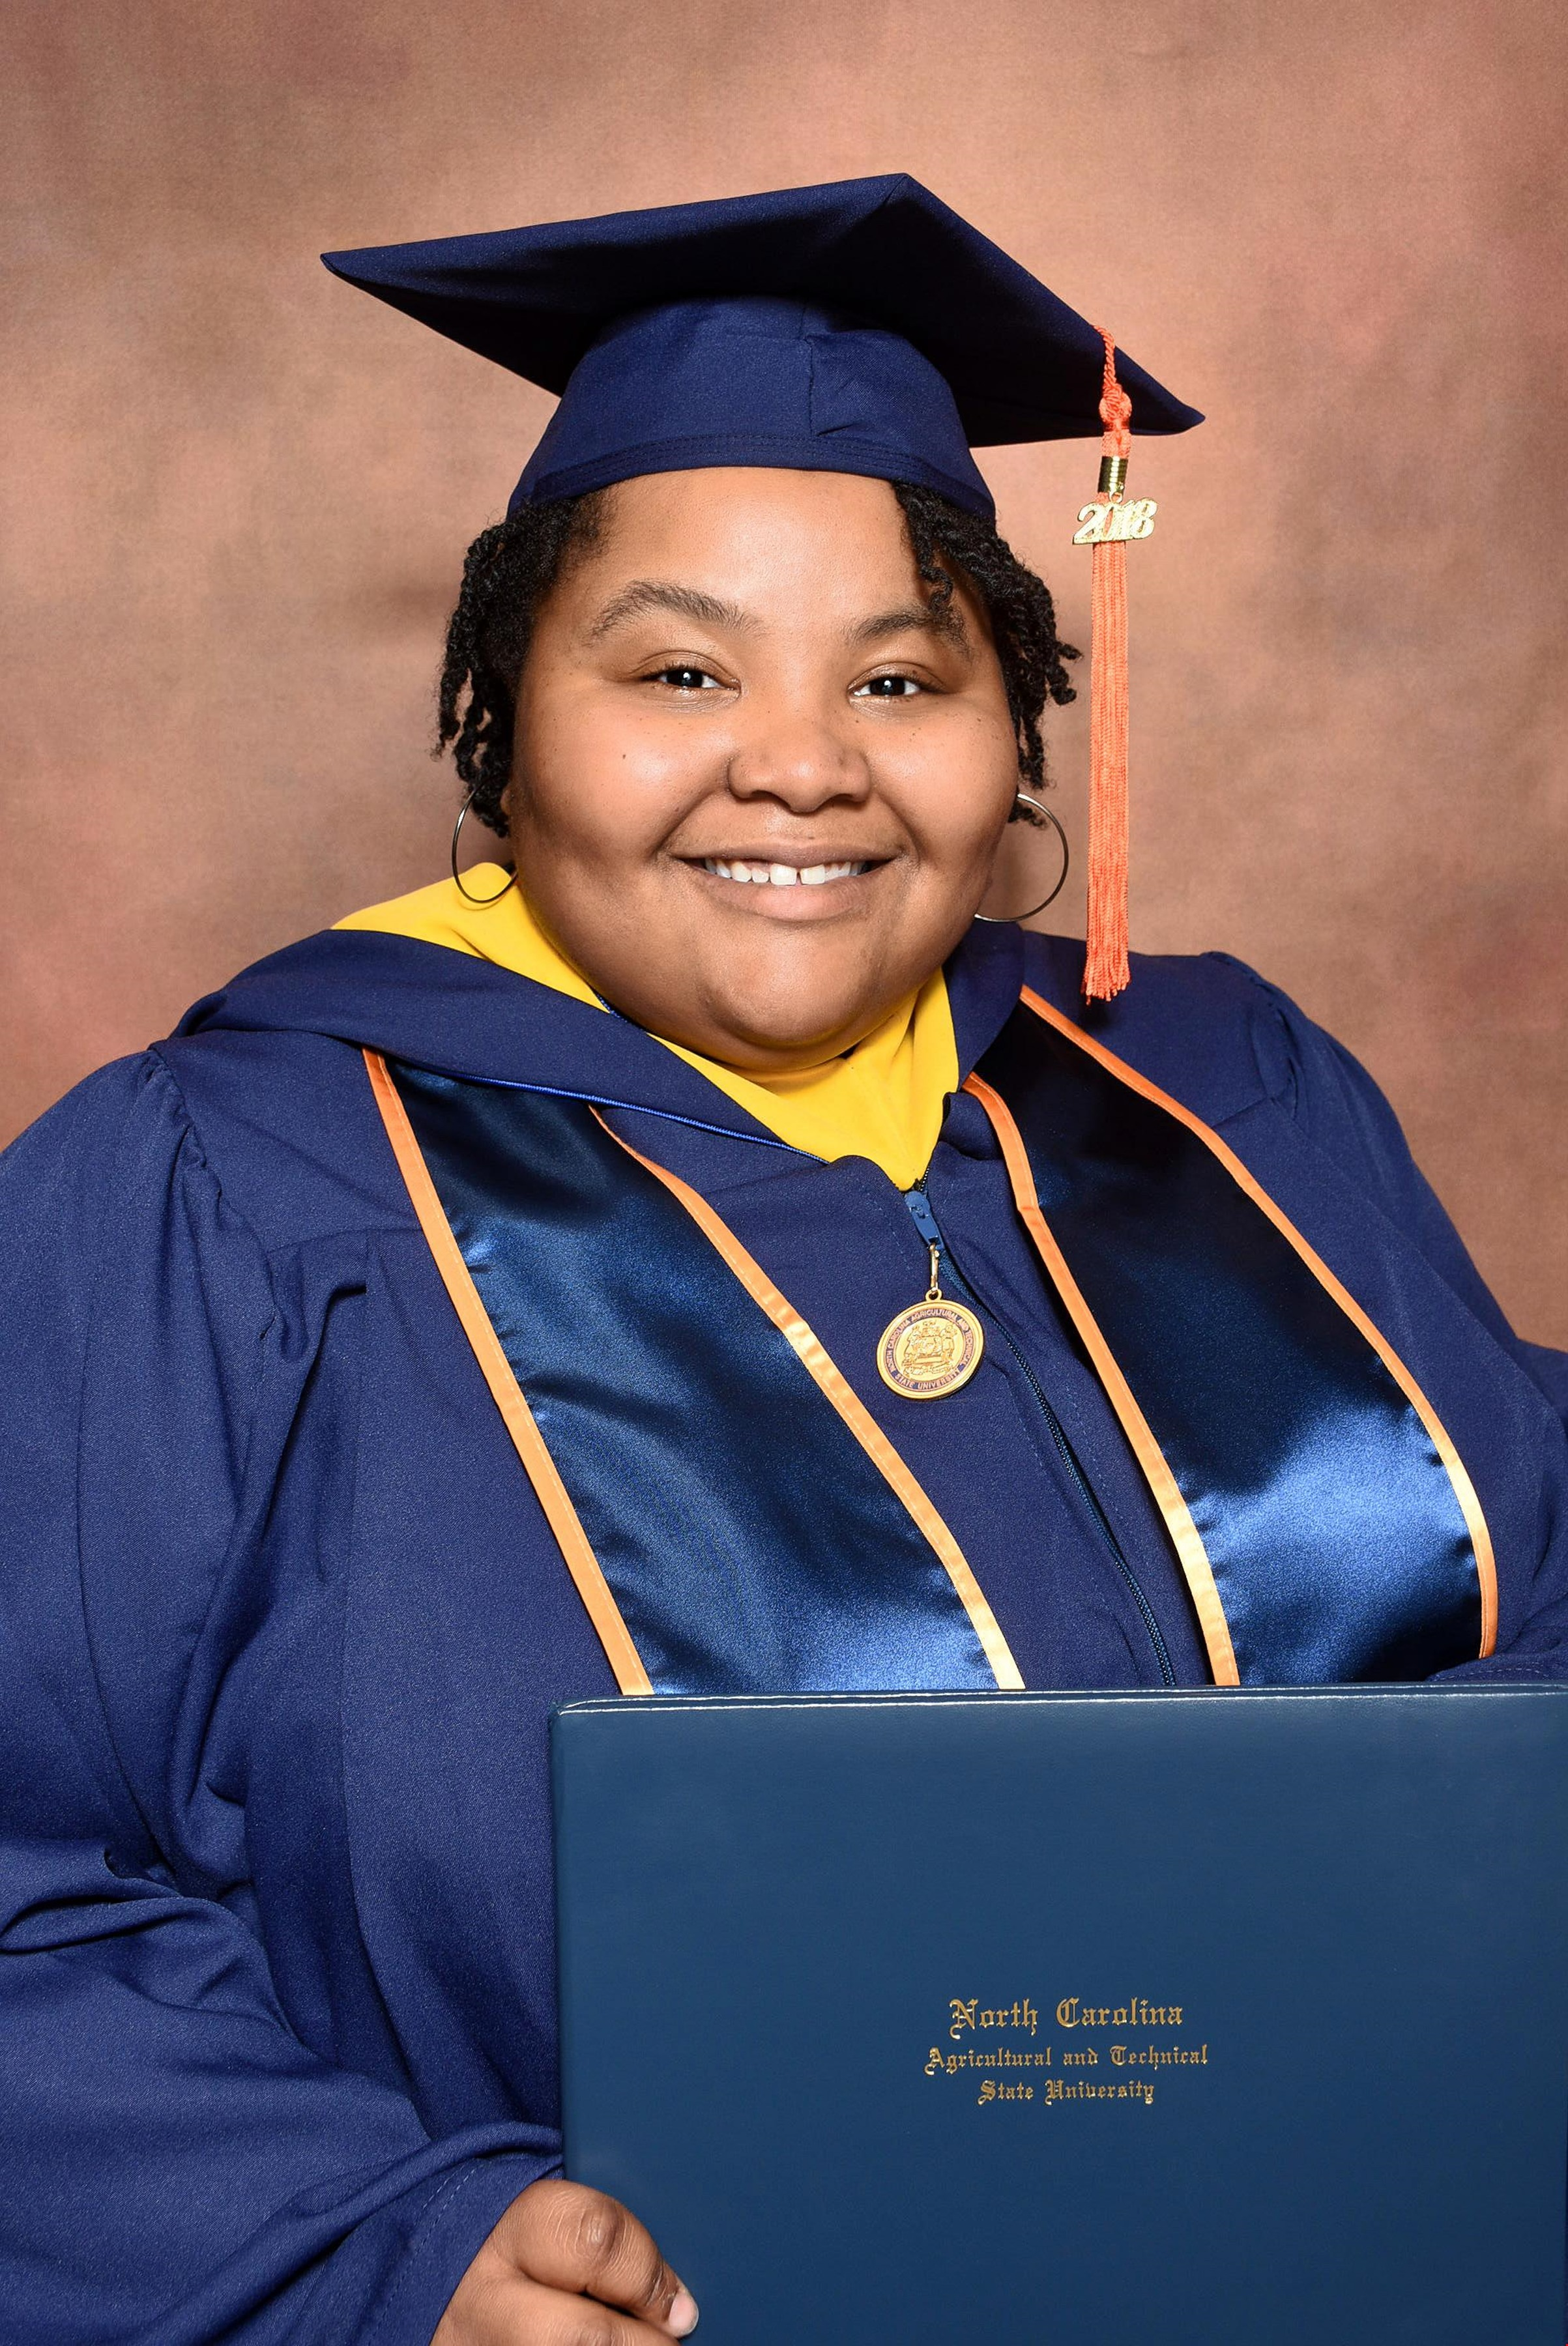
\includegraphics[width= 1in, height= 1.5in]{RosemondGrad.jpg}
    \caption{Photo of the author, Katrina Rosemond.}
\end{figure}

By enrolling in CS 6000, I aim to improve my research skills and 
understand who I am as a researcher. While I have been contributing to 
research projects since undergrad, I still struggle when I lead my 
projects. Mainly when writing, I never knew how much writing was involved 
when I first started in tech. So when I have to write a paper, I struggle 
with determining what's a good paper, pulling out the necessary 
information, and delivering that information on paper. But I know that the 
more I practice, the more I become comfortable with something. Therefore, 
I hope that between the lessons and assignments in CS 6000, I will learn 
to become a better scientific writer and more comfortable when I need to 
write a research paper.

\section{Git Repo}
The synCAN git repo \url{https://github.com/etas/SynCAN} is a synthetic 
controller area network (CAN) dataset used for CAN intrusion detection 
systems (IDSs). I'm currently researching the quality of CAN IDS datasets.

\section{Questions}
\textbf{Question 1:}
Hi Katrina, what is your PhD about, what kind of project are you currently pursuing?
\newline
\textbf{Answer 1:} I'm currently working on security mechanisms for automotive networks and while I don't have a specific question ready for my dissertation I plan on continuing my work in this area.  
\newline
\textbf{Question 2:}
Hi Katrina, what is your favorite part of your research on cyber-physical systems?
\newline
\textbf{Answer 2:}
\newline
\textbf{*FOR THOSE WHO WILL ADD TO THE DOCUMENT PLEASE REMOVE THE 'BEGIN' AND 'END' PREAMBLES OR THE REST OF DOCUMENT WILL NOT SHOW*}
